\chapter{STRING $\in$ NP}

Now we will take a look at recognition of STRING graphs. Mainly that this problem is indeed in NP. We have already shown in the first part that STRING-recognition is NP-hard. The main problem is that some string graphs require representation with exponentially many crossings. Which is not possible to guess in an NP algorithm.

Also we have shown (Schaeffer and Štěfanovič) result that any string graph has a representation with at most exponentially many crossings.

Before we continue lets give us an example of a graph and its STRING representation which can be seen on Fig. \ref{string example}.

\begin{figure}[!ht]\centering
	\begin{subfigure}{.45\textwidth}\centering
		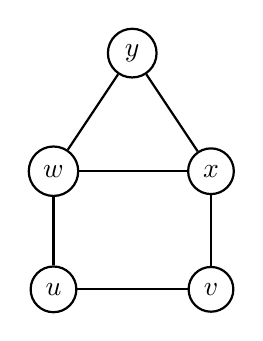
\begin{tikzpicture}[main/.style = {draw, circle, thick}]
			\node[main] (u) at (0,0) {$u$};
			\node[main] (v) at (2,0) {$v$};
			\node[main] (w) at (0,1.5) {$w$};
			\node[main] (x) at (2,1.5) {$x$};
			\node[main] (y) at (1,3) {$y$};
			\draw[thick] (u) -- (v);
			\draw[thick] (u) -- (w);
			\draw[thick] (v) -- (x);
			\draw[thick] (w) -- (x);
			\draw[thick] (w) -- (y);
			\draw[thick] (x) -- (y);
		\end{tikzpicture}
		\caption{Graph $G$.}
	\end{subfigure}
	\begin{subfigure}{.45\textwidth}\centering
		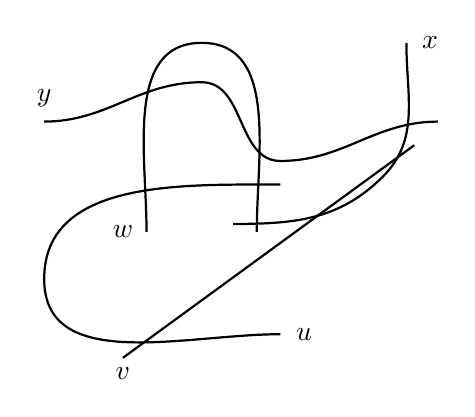
\begin{tikzpicture}
			\draw[thick] (-1,0) to[out=0, in=180] (1,.5) to[out=0, in=180] (2,-.5) to[out=0, in=180] (4,0);
			\node at (-1,.3) {$y$};
			\draw[thick] (.3, -1.4) to[out=90, in=180] (1,1) to[out=0, in=90] (1.7, -1.4);
			\node at (0, -1.4) {$w$};
			\draw[thick] (2, -0.8) to[out=180, in=90] (-1, -2) to[out=270, in=180] (2, -2.7);
			\node at (2.3, -2.7) {$u$};
			\draw[thick] (1.4, -1.3) to[out=0, in=225] (3.3, -.7) to[out=45, in=270] (3.6, 1);
			\node at (3.9, 1) {$x$};
			\draw[thick] (0, -3) to (3.7, -.3);
			\node at (0, -3.2) {$v$};
		\end{tikzpicture}
		\caption{String representation.}
	\end{subfigure}
	\caption{Example of a STRING graph.}
	\label{string example}
\end{figure}

Firstly lets define another problem which can be converted from STRING-recognition.

\section{Weak AT-realization}

The \textbf{INPUT} is a graph $G = (V,E)$ and $R \subseteq \binom{E}{2}$. The \textbf{GOAL} is to find a drawing of $G$ where only the pairs of edges from $R$ are allowed to cross.

Note that AT stands for abstract topological and weak means that the pairs do \textbf{not hove} to cross, only they can.

For now the drawing is somewhat basic. That is No edges crosses through a vertex. Vertices are points and edges are curves.

\section{Reduction of STRING-recognition to Weak AT-realization}

For a given graph $G = (V_G,E_G)$ we define the following graph $H = (V_H, E_H)$ and $R$. $V_H = V_G \cup E_G$ and $E_H = \{\{v,e\}, v \in V_G, e \in E_G, v \in e\}$. Lets see an example on Fig. \ref{reduction of strings}. We may see that the graph is obtained by subdividing all edges.

\begin{figure}[!ht]\centering
	\begin{subfigure}{.45\textwidth}\centering
		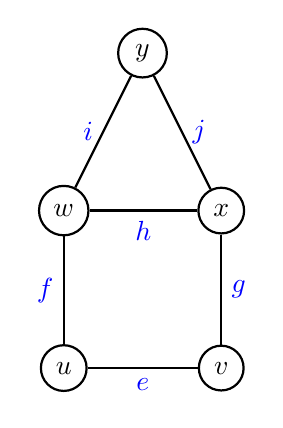
\begin{tikzpicture}[main/.style = {draw, circle, thick}, e/.style = {Blue}]
			\node[main] (u) at (0,0) {$u$};
			\node[main] (v) at (2,0) {$v$};
			\node[main] (w) at (0,2) {$w$};
			\node[main] (x) at (2,2) {$x$};
			\node[main] (y) at (1,4) {$y$};
			\draw[thick] (u) -- (v) node[midway, e, below] {$e$};
			\draw[thick] (u) -- (w) node[midway, e, left] {$f$};
			\draw[thick] (v) -- (x) node[midway, e, right] {$g$};
			\draw[thick] (w) -- (x) node[midway, e, below] {$h$};
			\draw[thick] (w) -- (y) node[midway, e, above, left] {$i$};
			\draw[thick] (x) -- (y) node[midway, e, above, right] {$j$};
		\end{tikzpicture}
		\caption{Original graph $G$.}
	\end{subfigure}
	\begin{subfigure}{.45\textwidth}\centering
		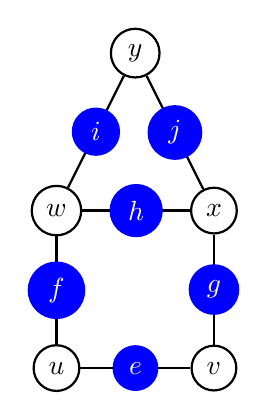
\begin{tikzpicture}[main/.style = {draw, circle, thick}, e/.style = {draw, circle, fill, Blue}]
			\node[main] (u) at (0,0) {$u$};
			\node[main] (v) at (2,0) {$v$};
			\node[main] (w) at (0,2) {$w$};
			\node[main] (x) at (2,2) {$x$};
			\node[main] (y) at (1,4) {$y$};
			\draw[thick] (u) -- (v) node[midway, e] {\textcolor{white}{$e$}};
			\draw[thick] (u) -- (w) node[midway, e] {\textcolor{white}{$f$}};
			\draw[thick] (v) -- (x) node[midway, e] {\textcolor{white}{$g$}};
			\draw[thick] (w) -- (x) node[midway, e] {\textcolor{white}{$h$}};
			\draw[thick] (w) -- (y) node[midway, e] {\textcolor{white}{$i$}};
			\draw[thick] (x) -- (y) node[midway, e] {\textcolor{white}{$j$}};
		\end{tikzpicture}
		\caption{Graph $H$.}
	\end{subfigure}
	\caption{Creating $H$ from $G$.}
	\label{reduction of strings}
\end{figure}

Lastly we define $R = \{\{\{v, e\}, \{w,f\}\}, \{v,w\} \in E_G\}$.

\begin{claim}
	$G$ is a STRING graph $\Leftrightarrow$ $(H,R)$ has Weak AT-realization.
\end{claim}

\begin{proof}
	"$\Rightarrow$" Suppose $G$ is a STRING graph. Pick endpoints as vertices and crossings as edge-vertices of $H$. Choose these arbitrary (see Fig. \ref{rightarrow} for an example). The edges will follow the lines in a STRING representation.
	
	"$\Leftarrow$" Suppose $(H,R)$ has a Weak AT-realization. See that $H$ is bipartite. Now represent it by going from the vertex alongside every edge to the edge-vertices of $H$ and almost return to the vertex. See Fig. \ref{leftarrow} for an example. It is easily observable that when lines cross then indeed they need be connected by an edge.
	
	\begin{figure}[!ht]\centering
		\begin{subfigure}{.4\textwidth}\centering
				\begin{tikzpicture}[main/.style = {draw, circle, thick, Blue}, c/.style = {thick, Blue},
					side/.style = {draw, circle, thick, Green}]
					\draw[c,name path=A] (-1,0) to[out=0, in=180] (1,.5) to[out=0, in=180] (2,-.5) to[out=0, in=180] (4,0);
					\node[main] at (-1.35,0) (y) {$y$};
					\draw[c,name path=B] (.3, -1.4) to[out=90, in=180] (1,1) to[out=0, in=90] (1.7, -1.4);
					\node[main] at (.3, -1.75) (w) {$w$};
					\draw[c,name path=C] (2, -0.8) to[out=180, in=90] (-1, -2) to[out=270, in=180] (2, -2.7);
					\node[main] at (2.35, -2.7) (u) {$u$};
					\draw[c,name path=D] (1.4, -1.3) to[out=0, in=225] (3.3, -.7) to[out=45, in=270] (3.6, 1);
					\node[main] at (3.6, 1.35) (x) {$x$};
					\draw[c,name path=E] (0, -3) to (3.7, -.3);
					\node[main] at (-.2, -3.25) (v) {$v$};
					% Intersections and dots
					\coordinate[name intersections={of=A and B, by=ab}];
					\fill[Green] (ab) circle (2pt) node[circle,draw] {};
					\coordinate[name intersections={of=A and D, by=ad}];
					\fill[Green] (ad) circle (2pt) node[circle,draw] {};
					\coordinate[name intersections={of=B and C, by=bc}];
					\fill[Green] (bc) circle (2pt) node[circle,draw] {};
					\coordinate[name intersections={of=B and D, by=bd}];
					\fill[Green] (bd) circle (2pt) node[circle,draw] {};
					\coordinate[name intersections={of=C and E, by=ce}];
					\fill[Green] (ce) circle (2pt) node[circle,draw] {};
					\coordinate[name intersections={of=D and E, by=de}];
					\fill[Green] (de) circle (2pt) node[circle,draw] {};
					\draw[dashed, thick, Green, bend right = 10] (v) edge (ce);
					\draw[dashed, thick, Green, bend left = 10] (u) edge (ce);
					\draw[dashed, thick, Green, bend right = 10] (v) edge (de);
					\draw[dashed, thick, Green, bend left = 10] (w) edge (bc);
					\draw[dashed, thick, Green, bend left = 10] (x) edge (ad);
				\end{tikzpicture}
			\caption{$\Rightarrow$ (Only some edges are present.)}
			\label{rightarrow}
		\end{subfigure}
		\begin{subfigure}{.58\textwidth}\centering
			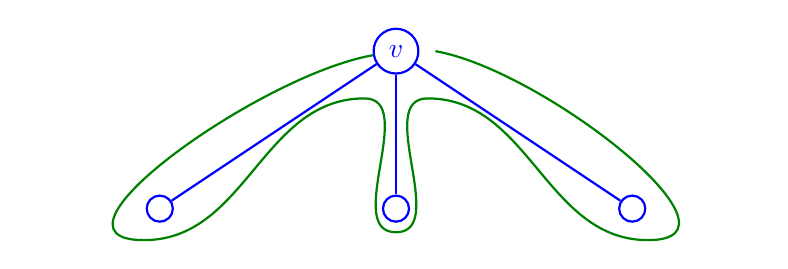
\begin{tikzpicture}[main/.style = {draw, circle, thick, Blue}]
				\node[main] at (0,0) (v) {$v$};
				\node[main] at (-3, -2) (1) {};
				\node[main] at (0, -2) (2) {};
				\node[main] at (3, -2) (3) {};
				\draw[thick, Blue] (v) to[] (1);
				\draw[thick, Blue] (v) to[] (2);
				\draw[thick, Blue] (v) to[] (3);
				\draw[thick, Green] (v) to[out=190, in=180] (-3.2, -2.4) to[out=0, in=180] (-.4,-.6) to[out=0, in=180] (0, -2.3) to[out=0, in=180] (.4,-.6) to[out=0, in=180] (3.2, -2.4) to[out=0, in=-10] (.5, 0);
			\end{tikzpicture}
			\caption{$\Leftarrow$}
			\label{leftarrow}
		\end{subfigure}
		\caption{Examples for the proof.}
	\end{figure}
\end{proof}

\subsection{Test Weak AT-realization in NP}

Firstly we will write down all our assumption about the drawing we will be using.

\begin{enumerate}
	\item We are on the sphere.
	\item Vertex $v$ is drawn as an open disc $D_v$ (also we will denote $\partial D_v$ as the boundary of $D_v$ and $\overline{D_v}$ as the closure of $D_v$, i.e. $\overline{D_v} = D_v \cup \partial D_v$).
	\item An edge $e = \{v,w\}$ is represented by a curve $\gamma_e$ connecting a point from $\partial D_v$ to a point from $\partial D_w$ otherwise $\gamma_e$ is disjoint from $\bigcup_{x \in V} \overline{D_x}$.
	\item For $e \neq f$ $\gamma_e$ and $\gamma_f$ have distinct endpoints.
\end{enumerate}

We can easily see that these assumption are not restricting since it can be switch to "normal" drawing we are using by shrinking the discs to single points and switch back by expanding the single points.

Now we will proceed with the algorithm.

\begin{algorithm}[!ht]
	\begin{algorithmic}[1]
		\Require $G = (V,E), R \subseteq \binom{E}{2}$
		\State $\forall v \in V:$ choose $D_v$ (so that $v \neq w$ have $\overline{D_v} \cap \overline{D_w} = \emptyset$).
		\State For any edge $e \in E$ incident to $v \in V:$ choose an endpoint of $\gamma_e$ on $\partial D_v$.
		\State \textcolor{Green}{$\dots$}
	\end{algorithmic}
	\caption{NP algorithm for testing Weak AT-realization.}
\end{algorithm}

Before we continue with the algorithm we will take a short topological detour to some definitions and facts.

\subsection{Topological detour}

\begin{defn}
	$\mathcal{S} := (\text{sphere}) \setminus \bigcup_{v \in V} D_v$. Which is a compact surface with boundary.
\end{defn}

\begin{defn}
	$\mathcal{S}-\text{curve}$ is a curve in $\mathcal{S}$ with endpoints in the $\partial \mathcal{S}$ and no other point in $\partial \mathcal{S}$.
\end{defn}

\begin{defn}
	Two $\mathcal{S}$-curves $\gamma, \delta$ are \textbf{isotopic} (written as $\gamma \sim \delta$) if $\gamma$ and $\delta$ have the same endpoints and $\gamma$ can be transformed into $\delta$ by a continuous deformations of $\mathcal{S}$ which fixes the boundary.
\end{defn}

\begin{figure}[!ht]\centering
	\begin{subfigure}{.45\textwidth}\centering
		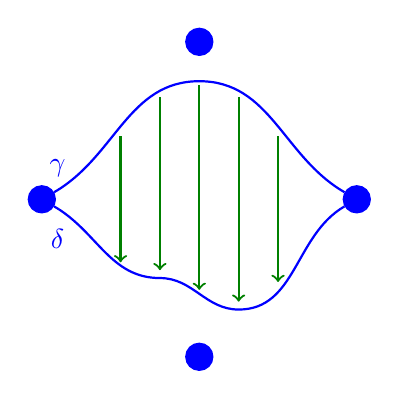
\begin{tikzpicture}[main/.style = {draw, circle, thick, fill, Blue}]
			\node[main] (0) at (0,2) {};
			\node[main] (1) at (-2,0) {};
			\node[main] (2) at (2,0) {};
			\node[main] (3) at (0, -2) {};
			\draw[thick, Blue] (1) to[out=30, in=180] (0,1.5) to[out=0, in=150] (2);
			\node[blue] (gamma) at (-1.8, .4) {$\gamma$};
			\draw[thick, Blue] (1) to[out=-30, in=180] (-.5,-1) to[out=0, in=180] (.5, -1.4) to[out=0, in=210] (2);
			\node[blue] (delta) at (-1.8, -.5) {$\delta$};
			\draw[thick, Green, ->] (0, 1.45) to[] (0,-1.15);
			\draw[thick, Green, ->] (-1, .8) to[] (-1,-.8);
			\draw[thick, Green, ->] (-.5, 1.3) to[] (-.5,-.9);
			\draw[thick, Green, ->] (.5, 1.3) to[] (.5,-1.3);
			\draw[thick, Green, ->] (1, .8) to[] (1,-1.05);
		\end{tikzpicture}
		\caption{Example of $\mathcal{S}$-curves $\gamma, \delta$ that are isotopic.}
	\end{subfigure}
	\begin{subfigure}{.45\textwidth}\centering
		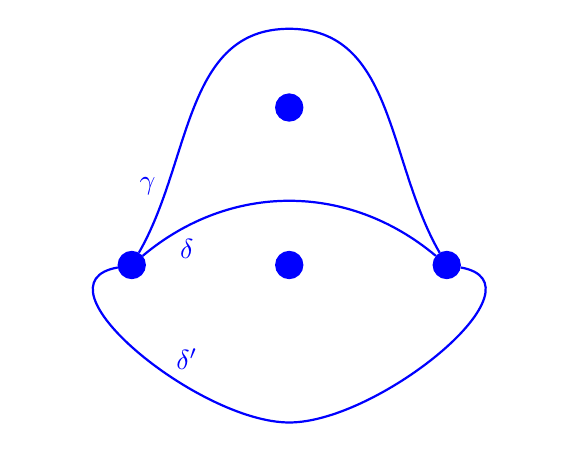
\begin{tikzpicture}[main/.style = {draw, circle, thick, fill, Blue}]
			\node[main] (0) at (0,2) {};
			\node[main] (1) at (-2,0) {};
			\node[main] (2) at (2,0) {};
			\node[main] (3) at (0, 0) {};
			\draw[thick, Blue] (1) to[out=40, in=140] (2);
			\node[blue] (gamma) at (-1.8, 1) {$\gamma$};
			\draw[thick, Blue] (1) to[out=60, in=180] (0,3) to[out=0, in=120] (2);
			\node[blue] (delta) at (-1.3, .2) {$\delta$};
			\draw[thick, Blue] (1) to[out=190, in=180] (0,-2) to[out=0, in=350] (2);
			\node[blue] (deltap) at (-1.3, -1.2) {$\delta'$};
		\end{tikzpicture}
		\caption{Counterexample of non-isotopic $\gamma \not \sim \delta$ and example of isotopic $\gamma \sim \delta'$.}
	\end{subfigure}
	\caption{Example of isotopic and non-isotopic $\mathcal{S}$-curves.}
\end{figure}

\begin{defn}
	For two $\mathcal{S}$-curves $\gamma_1, \gamma_2$ the intersection number $i(\gamma_1, \gamma_2)$ is
	
	$$
	\min_{\delta_1 \sim \gamma_1, \delta_2 \sim \gamma_2} |\delta_1 \cap \delta_2|.
	$$
\end{defn}

\begin{fact}
	Let $\gamma_1, \dots, \gamma_n$ be $\mathcal{S}$-curves. Then there are $\mathcal{S}$-curves $\delta_1, \dots, \delta_n$ s.t.
	
	\begin{enumerate}
		\item $\delta_i \sim \gamma_i$ for $i = 1, \dots, n$,
		\item $|\delta_i \cap \delta_j| = i(\gamma_i, \gamma_j)$ for $i\neg j \in \{1, \dots, n\}$. 
	\end{enumerate}
\end{fact}

\noindent
With all these definitions we will choose the following triangulation $T = (V_T, E_T)$ of $\mathcal{S}$:

\begin{enumerate}
	\item $\forall v \in V: \partial D_v$ has three vertices and three edges of $T$.
	\item There are no other vertices of $T$, the remaining edges are chosen arbitrarily as $\mathcal{S}$-curves, so that $\mathcal{S}$ is partitioned into triangle faces.
	\item Vertices of $T$ do not coincide with endpoints of $\gamma_e, e \in E$ from algorithm.
\end{enumerate}

\begin{defn}
	An $\mathcal{S}$-curve $\gamma$ is \textbf{normal} w.r.t. T if
	
	\begin{enumerate}
		\item The endpoints of $\gamma$ are distinct from $V_T$.
		\item Any point where an edge of $T$ meets $\gamma$ is either an endpoint of $\gamma$ or a proper crossing (no touching is allowed).
		\item $\gamma$ does not have two consecutive crossings with any edge of $T$.
		\item $\gamma$ does not cross the same edge of $T$ no more than $2^{|E_T| + |E|}$-times.
	\end{enumerate}
\end{defn}

\begin{claim}
	If $G$ has a weak AT-realization, then it has a realization where each $\gamma_e$ is normal w.r.t. T.
\end{claim}

\begin{proof}
	Take AT with minimum number of crossings. 1. is satisfied by the definition. 2. otherwise minimality is broken, 3. again the minimality is broken and lastly 4. follows from GRG1.
	
	\begin{figure}[!ht]\centering
		\begin{subfigure}{.2\textwidth}\centering
			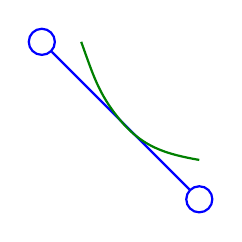
\begin{tikzpicture}[main/.style = {draw, circle}, e/.style = {thick, Blue}]
				\node[main,e] at (0,0) (0) {};
				\node[main,e] at (-2,2) (1) {};
				\draw[e] (0) -- (1);
				\draw[thick, Green] (0, .5) to[out=170, in=310] (-1,1) to[out=130,in=290] (-1.5,2);
			\end{tikzpicture}
			\caption{Second before.}
		\end{subfigure}
		\begin{subfigure}{.2\textwidth}\centering
			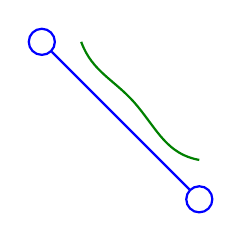
\begin{tikzpicture}[main/.style = {draw, circle}, e/.style = {thick, Blue}]
				\node[main,e] at (0,0) (0) {};
				\node[main,e] at (-2,2) (1) {};
				\draw[e] (0) -- (1);
				\draw[thick, Green] (0, .5) to[out=170, in=310] (-.8,1.2) to[out=130,in=290] (-1.5,2);
			\end{tikzpicture}
			\caption{Second after.}
		\end{subfigure}
		\begin{subfigure}{.2\textwidth}\centering
			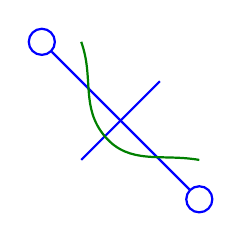
\begin{tikzpicture}[main/.style = {draw, circle}, e/.style = {thick, Blue}]
				\node[main,e] at (0,0) (0) {};
				\node[main,e] at (-2,2) (1) {};
				\draw[e] (0) -- (1);
				\draw[e] (-1.5,.5) -- (-.5,1.5);
				\draw[thick, Green] (0, .5) to[out=170, in=310] (-1.2,.8) to[out=130,in=290] (-1.5,2);
			\end{tikzpicture}
			\caption{Third before.}
		\end{subfigure}
		\begin{subfigure}{.2\textwidth}\centering
			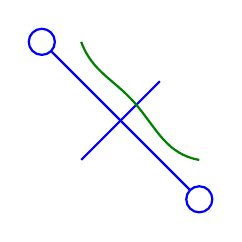
\begin{tikzpicture}[main/.style = {draw, circle}, e/.style = {thick, Blue}]
				\node[main,e] at (0,0) (0) {};
				\node[main,e] at (-2,2) (1) {};
				\draw[e] (0) -- (1);
				\draw[e] (-1.5,.5) -- (-.5,1.5);
				\draw[thick, Green] (0, .5) to[out=170, in=310] (-.8,1.2) to[out=130,in=290] (-1.5,2);
			\end{tikzpicture}
			\caption{Third after.}
		\end{subfigure}
		\caption{Examples for the proof.}
	\end{figure}
\end{proof}

\begin{defn}
	Let $\gamma$ be an $\mathcal{S}$-curve, normal w.r.t T for $e \in E_T: C_e(\gamma) := |e \cap \gamma|$.
\end{defn}

\begin{claim}
	The numbers $\left( C_e(\gamma)\right)_{e \in E_T}$ determine $\gamma$ up to isotopy.
\end{claim}

\begin{proof}
	Suppose we have a triangle face.
\end{proof}